\documentclass{article}
\usepackage{tikz}
\usetikzlibrary{shapes.multipart, positioning, arrows.meta, shapes.geometric, calc}
\usepackage[margin=0.5in]{geometry}

\begin{document}
\begin{figure}[htbp]
\centering
\resizebox{\textwidth}{!}{
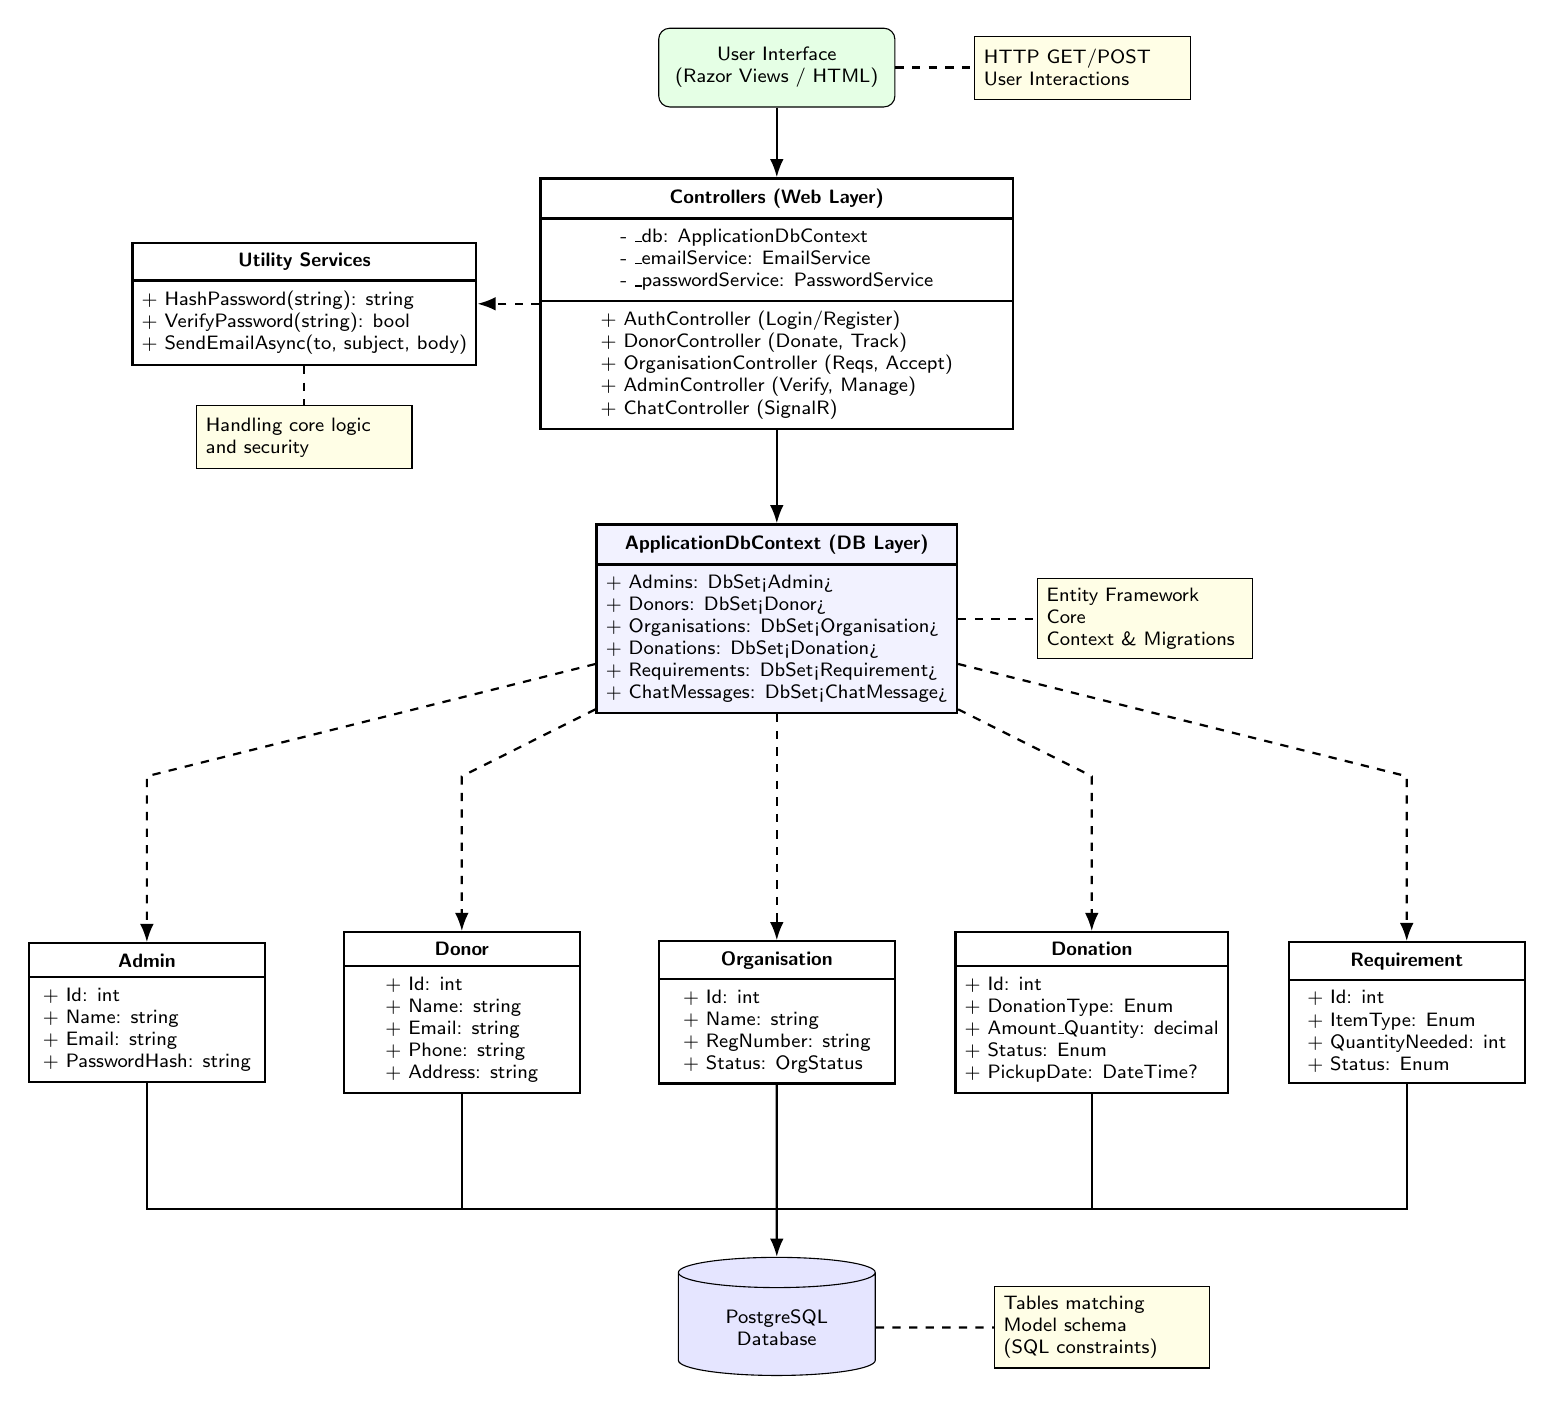
\begin{tikzpicture}[
    >=Latex,
    font=\sffamily\scriptsize,
    class/.style={
        draw, rectangle split, rectangle split parts=2,
        minimum width=3cm, align=left, fill=white, thick
    },
    interface/.style={
        draw, rectangle split, rectangle split parts=2,
        minimum width=2.5cm, align=left, fill=gray!10, thick
    },
    note/.style={
        draw, rectangle, fill=yellow!10, minimum height=0.8cm, align=left, text width=2.5cm
    },
    db/.style={
        draw, cylinder, shape border rotate=90, aspect=0.25,
        minimum width=2.5cm, minimum height=1.5cm, fill=blue!10, align=center
    },
    ui/.style={
        draw, rounded corners, fill=green!10, minimum width=3cm, minimum height=1cm, align=center
    },
    line/.style={draw, thick, -},
    dashedline/.style={draw, thick, dashed, -},
    arrow/.style={draw, thick, ->},
    dashedarrow/.style={draw, thick, dashed, ->},
    implement/.style={draw, thick, dashed, -{Triangle[open, scale=1.5]}}
]

% ==========================================
% TOP LEVEL: UI & INTERFACES
% ==========================================

\node[ui] (UI) at (0, 10) {User Interface \\ (Razor Views / HTML)};

\node[note] (UINote) [right=1cm of UI] {HTTP GET/POST \\ User Interactions};
\draw[dashedline] (UI) -- (UINote);

% ==========================================
% CONTROLLER LAYER (Equivalent to Service logic)
% ==========================================

\node[class, rectangle split parts=3, minimum width=6cm] (Controllers) at (0, 7) {
    \textbf{Controllers (Web Layer)}
    \nodepart{second}
    - \_db: ApplicationDbContext \\
    - \_emailService: EmailService \\
    - \_passwordService: PasswordService
    \nodepart{third}
    + AuthController (Login/Register) \\
    + DonorController (Donate, Track) \\
    + OrganisationController (Reqs, Accept) \\
    + AdminController (Verify, Manage) \\
    + ChatController (SignalR)
};

\draw[arrow] (UI) -- (Controllers);

% Services
\node[class] (Services) at (-6, 7) {
    \textbf{Utility Services}
    \nodepart{second}
    + HashPassword(string): string \\
    + VerifyPassword(string): bool \\
    + SendEmailAsync(to, subject, body)
};

\node[note] (ServiceNote) [below=0.5cm of Services] {Handling core logic \\ and security};
\draw[dashedline] (Services) -- (ServiceNote);

\draw[dashedarrow] (Controllers) -- (Services);

% ==========================================
% DATA ACCESS LAYER
% ==========================================

\node[class, minimum width=4cm, fill=blue!5] (DBLayer) at (0, 3) {
    \textbf{ApplicationDbContext (DB Layer)}
    \nodepart{second}
    + Admins: DbSet<Admin> \\
    + Donors: DbSet<Donor> \\
    + Organisations: DbSet<Organisation> \\
    + Donations: DbSet<Donation> \\
    + Requirements: DbSet<Requirement> \\
    + ChatMessages: DbSet<ChatMessage>
};

\draw[arrow] (Controllers) -- (DBLayer);

\node[note] (DBNote) [right=1cm of DBLayer] {Entity Framework Core \\ Context \& Migrations};
\draw[dashedline] (DBLayer) -- (DBNote);

% ==========================================
% MODELS LAYER
% ==========================================
% Arranged horizontally to match the reference style

\node[class] (AdminModel) at (-8, -2) {
    \textbf{Admin}
    \nodepart{second}
    + Id: int \\
    + Name: string \\
    + Email: string \\
    + PasswordHash: string
};

\node[class] (DonorModel) at (-4, -2) {
    \textbf{Donor}
    \nodepart{second}
    + Id: int \\
    + Name: string \\
    + Email: string \\
    + Phone: string \\
    + Address: string
};

\node[class] (OrgModel) at (0, -2) {
    \textbf{Organisation}
    \nodepart{second}
    + Id: int \\
    + Name: string \\
    + RegNumber: string \\
    + Status: OrgStatus
};

\node[class] (DonationModel) at (4, -2) {
    \textbf{Donation}
    \nodepart{second}
    + Id: int \\
    + DonationType: Enum \\
    + Amount\_Quantity: decimal \\
    + Status: Enum \\
    + PickupDate: DateTime?
};

\node[class] (ReqModel) at (8, -2) {
    \textbf{Requirement}
    \nodepart{second}
    + Id: int \\
    + ItemType: Enum \\
    + QuantityNeeded: int \\
    + Status: Enum
};

% Routing connections from DBLayer to Models
\draw[dashedarrow] (DBLayer) -- (-8, 1) -- (AdminModel.north);
\draw[dashedarrow] (DBLayer) -- (-4, 1) -- (DonorModel.north);
\draw[dashedarrow] (DBLayer) -- (OrgModel.north);
\draw[dashedarrow] (DBLayer) -- (4, 1) -- (DonationModel.north);
\draw[dashedarrow] (DBLayer) -- (8, 1) -- (ReqModel.north);

% ==========================================
% DATABASE LAYER
% ==========================================

\node[db] (PostgreSQL) at (0, -6) {PostgreSQL \\ Database};

\draw[line] (AdminModel.south) -- (-8, -4.5) -- (0, -4.5);
\draw[line] (DonorModel.south) -- (-4, -4.5) -- (0,-4.5);
\draw[line] (DonationModel.south) -- (4, -4.5) -- (0,-4.5);
\draw[line] (ReqModel.south) -- (8, -4.5) -- (0,-4.5);
\draw[arrow] (OrgModel.south) -- (PostgreSQL.north);

\node[note] (DbNote) [right=1.5cm of PostgreSQL] {Tables matching \\ Model schema \\ (SQL constraints)};
\draw[dashedline] (PostgreSQL) -- (DbNote);


\end{tikzpicture}
}
\caption{Comprehensive Architecture and Class Diagram (Layered Design)}
\end{figure}
\end{document}
